\documentclass[a4paper,11pt]{article}
\usepackage[T1]{fontenc}
\usepackage[utf8]{inputenc}
\usepackage{lmodern}
\usepackage{csquotes}

\usepackage{hyperref}
\usepackage{graphicx}
\usepackage[table]{xcolor}
\usepackage[english]{babel}
\usepackage[hashEnumerators]{markdown}

\usepackage{nameref}
\usepackage{graphicx}
\graphicspath{ {../Images/} }

% Defines how the section reference looks
\newcommand{\sectiondescribe}[1]{(Sektion {#1})}
\newcommand{\imagedescribe}[1]{(Bild {#1})}
\addto\captionsenglish{\renewcommand{\figurename}{Bild}}

\title{\Huge \textbf{Rovdjur i Norrbotten}}
\author{\textsc{Josef Utbult}}

\begin{document}
\pagenumbering{roman}
\maketitle
\newpage
\tableofcontents
\newpage
\pagenumbering{arabic}
%
\section{Bakgrund}
Luleå Universitet är (i det här fiktiva universumet) ett universitet som anlades utanför Luleå år 1886. De instutitioner som är främst aktiva här är Instutitionen för naturhistoria, där botanik och zoologi forskas om, Instutitionen för teknik, som syslar med mattematik, mekanik och fysik, och Instutitionen för filosofi, där allt mellan historia, religion, sammhälskunskap och konsthistoria studeras. Det mycket få vet om är att det även finns en till instutition, Instutitionen för signeri- och rationelt avvikande teknik, som sysslar med att dokumentera det okulta, studerar \textit{taumaturgi} (Läran om magi, ritualer och transmutation) samt samlar på övernaturliga artifakter och verk.

Äventyrarna i denna kampanj är alla studenter vid Luleå Universitet, och lär känna varandra igenom \textit{Anna Olofsson} \sectiondescribe{\ref{kar:AnnaOlofsson}}, en literaturstudent som också är ansvarig utgivare för \textit{Luleå studentkårs magasin}. Det hela börjar med att de blir inbjudna till Annas lägenhet på middag. Natten efter detta upplever alla äventyrare samma dröm, och när de väcks av en polis vid deras dörr får de reda på att Anna har funnits död, med stora klösmärken över hennes strupe...

\section{Äventyrets början}

\begin{displayquote}
	\textit{Luleå Universitet} är Norrlands metropol när det kommer till den akademiska världen. Trots att antalet bildade i den norra delen av Sverige är mycket låg, beslöt sig självaste \textit{Gustaf VI Adolf} att ett universitet ska byggas i Sveriges nordligare del. Detta för att underlätta både de biologiska studier som utförs på Norrlands flora och fauna, samt för att bidra med teknisk kompetens till alla närliggande industrier.

	Ni är några av de få som valt att flytta ända upp till denna avlägsna plats, för att studera vid detta universitet. Men för en kväll har ni alla valt att skjuta studierna åt sidan för att medverka på den middag som er vän bjudit er till. \textit{Anna Olofsson} är en ung dam som studerar literatur vid Luleå Universitet och är ansvarig utgivare för \textit{Luleå studentkårs magasin}, en tidsskrift ämnad åt studerande och anställda vid Luleå Universitet. Ni träffar alla varandra vid trappuppgången till hennes studentlägenhet.
\end{displayquote}

\subsection{Annas Middag}

Äventyrarna blir snart insläppta i Annas lägenhet, en tvåa med en kokvrå, ett vardagsrum och ett sovrum. De serveras en stek med potatis och kokta grönsaker och Anna börjar småprata. Hon nämner att hon haft sådana problem på tidningens kontor, de har fått en skokartong med en död råtta i levererat till deras antre. Hon misstänker att de är ``De satans ungarna från Porsöligan igen''. De har uppenbarligen trakaserat tidsskriftens arbetare flera gånger efter att de publicerat ett avslöjande som fick en av medlemmarna att hamna i fängelse. När äventyrarna lämnar Anna verkar hon sömnig, men ändå väldigt glad över sin middag. 

\subsection{Utanför Annas lägenhet}
När ni kommer ut från lägenheten är det mörkt ute. Det ni ser är upplyst av de gatulyktor som finns placerade på den gångväg som är upplyst runt det här kvarteret av lägenheter.

Alla utredare får slå ett slag för Finna dolda ting. Om denne lyckas med ett svårt slag kan de se en skugga, som snabbt hukar sig bakom en husvägg, ca 30 meter bort. Om utredarna springer mot skuggan, märker de snabbt att den individ som spionerat på dem är borta.

\subsection{Mordet}
Sedan när alla sover.

\begin{displayquote}
	Under natten kommer det till er en dröm. Ni befinner er alla, själv, i ett mörkt rum fullt av dimma. Ni ser ett stenlagt golv, som ni verkar stå hukande på, som att ni är helt utmattade. Ni kan inte urskilja hur de ser ut, men ni ser två skuggiga människor som ser ner på er. Den ena säger ``Sök vidare. Vad vet hon egentligen?''.

	Ni vaknar kallsvättiga av att någon knackar på ytterdörren.
\end{displayquote}
%
Utanför era dörrar står en poliskonstapel. Han hämtar utredarna en åt gången, och ber dem följa med honom till stationen. Börja med en utredare, där konstapeln plockar upp denne och sedan går till nästa utredare (med den första i följe), och fortsätt till alla utredare. Konstapeln introducerar sig som \textit{Carl Svidsstål} \sectiondescribe{\ref{kar:KonstapelCarlSvidstal}} och är mycket tydlig med att utredarna inte är annhållna, utan att detta endast är ett förhör. 

Utredarna leds alla till en bil (eller två) som för er till Luleås Polishus. Där förs de in i ett väl upplyst rum med ett bord och stolar. Konstapel Svidstål kommer snart in med en portfölj. Han ser alvarlig ut, men också något sorgsen ut.

Han undrar vart utredarna var igår, när de senast såg Anna Olofsson, och vad alla gjorde när det lämnat hennes lägenhet. Konstapeln berättar med en sorgsen röst att det skett ett mord, och att offret är utredarnas vän Anna. Han tar upp sin portfölj, och berättar för utredarna att de absolut inte måste se på de bilder han har, men att han förstår att det kan vara viktigt för att förstå allvaret i situationen.

\begin{displayquote}
	På den första bilden ser ni Annas kropp, livlös på en brits. Hennes vanligen så vackra ansikte är blekt och insjunket. Bilden inefattar hennes huvud ner till hennes bröstkorg, och ni kan se de fasansfulla snitt som går tvärs över hennes hals. Det är tre djupa sår som går parallelt med varandra, med ett mellanrum på tre centimeter mellan varje jack.

	Den andra bilden föreställer Annas ben, visat bakifrån. Man kan se ännu en skada, men här verkar det vara ett mycket större ingrepp. Baksidan av hennes lår är borta, och det som finns kvar är ett stort köttsår från nedre delen av hennes stjärt ner till hennes knäveck. Ni kan se att det blod som än gång pumpats igenom hennes värmande hjärta, nu har koagulerat och torkats bort. Det enda som syns är hennes kött och vitan av hennes lårben.
\end{displayquote}
%
Alla utredare som ser på bilden tappar 1/1T4 + 1 i sinneshälsa. 

Konstapel Svidsstål beklagar ypperligt, och säger till utredarna att de är fria att gå. Han uppmanar dock till att utredarna inte ska gå till bråttsplatsen, då Anna inte längre förvaras där. Ni skjutsas åter hem till era lägenheter.
\newpage
%
%
\section{Biblioteket}
I biblioteket jobbar en äldre dam vid namn Rosa Edensdag. Hon är lätt grinig, men kan hjälpa utredarna hitta vad de vill ha med en normalt lyckat slag för övertyga. Annars kan en utredare slå ett slag för bokföring och lyckas med ett normalt slag hitta professor Olofssons avhandlingar/böcker. Med ett slag för bokföring eller historia kan en utredare med ett svårt lyckat slag hitta följande, eller med ett normalt lyckat slag ifall denne vet vad den ska leta efter. I professorns bok \textit{Poro-, Leopard- och Krokodilsällskapet; Naturreligioner i Sierra Leon och nordöstra Afrika}.

\begin{displayquote}
	\textbf{Borfima}

	Enligt den svarte mannen kring Sierra Leon, är en borfima en typ av avbild använd av \textit{Leopardsälskapet}, till för att blidka en gud; i dessas fall deras \textit{Leopard-gud}. En borfima består av en påse oftast gjord i läder, men även övriga textiler har setts användas. Denne ska fyllas med blod, fett, äggvita, blodet av en tupp och ris. Enligt de medlemmar i sällskapet som lyckats övertalats att avslöja denna sekt, är dock det som krävs för att borfiman ska uppnå dennes fulla potential blod från ett mänskligt offer. Mer specifikt ska offret vara \textit{från bärarens kött}, helst en son eller dotter men övriga offer från familjen har även inträffat. När denna borfima fyllts på, det gruppen kallat att \textit{mata} borfiman, ska denne bringa lycka och makt åt innehavaren. En dåligt skött borfima ska däremot bringa olycka på hela dennes familj.

	Utdrag ur \textit{Poro-, Leopard- och Krokodilsällskapet; Naturreligioner i Sierra Leon och nordöstra Afrika}, Prof. T Olofsson.
\end{displayquote}

\newpage
%
\section{Brådmans Bar}
\label{loc:BradmansBar}
Bar. Möter några från porsöligan här. De tjafsar med Migel Chapdelain. Han har en dikt som leder dem till G Huset. Han tappar den ur sin rock när en av ligisterna kuffar till honom.

\newpage
%
\section{SRT}
\label{loc:SRT}
\textit{Institutionen för signeri- och rationellt avvikande teknik}, eller förkortat; SRT, är en sektion under Luleå Universitet som inte många känner till. Denna institution är dock en stor anledning till att universitetet över huvud taget finns till, då dess systerinstitution under Den Kungliga Tekniska Högskolan behövde en utpost i Norrland för att studera diverse fornlämningar och dylikt. Denna institution är belägrad i det som kallas \textit{G huset}, en katedral-liknande byggnad som ligger placerad i en dimensionell ficka på andra sidan vägen av C huset.
%
\subsection{Att ta sig till G huset}
\label{uppd:TaSigTillG}
För att ta sig till G huset krävs det att Utredarna utför en simpel ritual, bestående av att gå en specifik slinga mellan husen på universitetet. Denna slinga finns beskriven i form av en dikt på lappen som Professor Chapdelains tappar på Brådmans Bar \sectiondescribe{\ref{loc:BradmansBar}}. Dikten på lappen lyder.
%
\begin{displayquote}
\begin{center}
	\textit{Ut ur hus F en allé jag ser. \\
	Jag går åt det håll dit där solen går ner. \\
	\vspace*{10px}
	Tre fram, en höger och sedan två bak. \\
	När jag till sist går till vänster, \\
	är där tornet även idag.}
\end{center}
\end{displayquote}
%
För att ta sig till G huset måste Utredarna gå följande slinga.
%
\begin{enumerate}
	\item Utredarna börjar vid en av de två ingångarna till F huset som ligger på regnbågsallén.
	\item Utredarna rör sig längst med regnbågsallén till slutet av D huset.
	\item Utredarna går norr, runt kanten av D huset till dess baksida.
	\item Utredarna rör sig tillbaks på baksidan av alla hus till gångvägen mellan E huset och F huset.
	\item Utredarna går söderut, ner för gångvägen till parken som ligger söder om universitetet. 
\end{enumerate}
%
\subsection{G Huset}
Viker utredarna av från den specificerade vägen nollställs ritualen, och de måste åter igen börja från F huset. Om de kommer till vägen mellan E huset och F huset händer följande.
%
\begin{displayquote}
	När ni går runt hörnet och börjar gå längst vägen mellan E och F ser ni det gröna koppartaket av den katedralliknande byggnaden som ligger mitt emot A, bredvid den park där ni spenderat många sommardagar. Ni går förbi A och kommer fram till huset, en åldrande byggnad av svart tegel och stora färgade fönster, där ni möts av en mörkt blå metallisk obelisk. På denna står det en förkortning som ni inte vet vad den syftar på; SRT. Den stora porten in i byggnaden står stängd.
\end{displayquote}
%
Om någon av spelarna undrar vad det här egentligen är för byggnad, kan du be dem slå för historia eller navigera. Om de misslyckas med ett normalt slag tänker de att de inte har någon aning riktigt. Med ett lyckat normalt slag inser de att de verkligen borde veta och inte kan förstå varför de inte vet. Det är som att byggnaden alltid varit där, men att du aldrig har reflekterat över den.

Vid porten kan utredarna knacka på, försöka höra/se vad som pågår i byggnaden eller smita in. Trots att målet med ett rollspel är att utredarna ska få göra vad de vill, bör du inte släppa in dem i byggnaden, då det förstör mystiken något.

Försöker de lyssna hör de en man med fransk brytning diskutera högljutt med någon okänd. Ser de in igenom något fönster kan de lägga märke till att detta är Professor Chapdelain \sectiondescribe{\ref{kar:MigelChapdelain}} som språkar med någon som ser ut att vara en student.

Beroende på hur lång tid det tar för utredarna att göra något, kommer professorn snart ut ur byggnaden. Han hälsar förbryllat, på utredarna och frågar vad de gör där.

Ifall de frågar om byggnaden menar han att den alltid varit där, och låtsas inte förstå varför utredarna är såpass förvirrade. Frågar de om vad han gör där, säger han endast att de inte har med det att göra.

Pratar de dock om Anna, ser professorn fundersam ut, men räknar snabbt ut att detta är Professor Olofssons systerdotter. Han visste inte att det var hon som var mördad, och pusslar nu ihop att det antagligen har något att göra med hennes morbror. Han vill inte avslöja för mycket, men nämner att han länge varit misstänksam emot professorn.

Chapdelain föreslår att utredarna ska ta en närmare titt på professor Olofsson. Den konkreta informationen han kan ge är att utredarna bör prata med Servicedesk om att få den information som är publik angående professorn. De skulle även kunna kolla med skolans bibliotek om de har mer information angående hans professionella historia.

Börjar utredarna ställa till med oreda ropar professorn på några förbipasserande som kommer till hans undsättning. Detta gör att byggnaden försvinner när utredarna inte ser på den, och de förbipasserande ingriper.

\newpage
%
\section{Prof. Olofssons kontor}
\label{loc:OlofssonsKontor}
%
\begin{figure}[h]
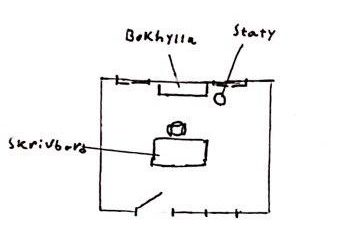
\includegraphics[width=8cm]{ProfOlofssonsKontor.png}
\centering
\end{figure}
%
Om utredarna kommer till Prof. Olofssons kontor den första dagen är inte professorn där, utan en handskriven lapp är fäst på hans dörr.

\begin{displayquote}
	Ursäkta min brådskande frånvaro, men av tragiska familjeskäl har jag blivit tvungen att ta tjänstledigt. Jag beklagar, då jag har nämnt för mina studenter att jag ska vara närvarande idag, samt ber jag om ursäkt för de möten som jag tvärt blivit tvungen att ställa in. Jag är dock åter igen imorgon under mina vanliga arbetstider.

	- Prof. Olofsson
\end{displayquote}
%
Om utredarna slår ett lyckat normalt slag för finna dolda ting kan de se en våt fläck på pappret som har torkat in. Kommer utredarna en senare dag är Prof. Olofsson på sitt kontor.

\begin{displayquote}
	När ni kommer till professor Olofssons kontor står dörren öppen. Där inne, vid ett skrivbord sitter en äldre man med grått hår, små glasögon och ett pipskägg. Han är klädd i en vit skjorta och kavajbyxor, och han verkar för närvarande läsa en bok. På väggarna hänger tavlor med orientaliska mönster och masker i både lera och trä. Fönstret i rummet är täckt i vackra tyger. Han har en stor bokhylla bakom sig, full med både böcker och andra föremål. Det är kompasser, små målade stenar, armband och flätade korgar. Rummet luktar något unket och instängt. Bredvid bokhyllan står även en staty i sten, föreställande en mans kropp, men med ett leopardhuvud.
\end{displayquote}
%
Prof. Olofsson \sectiondescribe{\ref{kar:TomasOlofsson}} verkar vara en mycket artig man, och hälsar vänligt på utredarna. Han säger att han gladligen pratar med studenter så ofta han får möjlighet, och alltid försöker vara till hjälp. Om utredarna slår ett lyckat normalt inteligensslag emot professorn, noterar de att hans skjorta verkar ostruken och hans kavajbyxor verkar inte ha pressats på ett tag. Frågar utredarna om Anna berättar professorn följande.

\begin{displayquote}
	Ni ser plötsligt hur professorns annars muntra uttryck blir dystert och allvarsamt.
	``Jaså ni är vänner till Anna. Jag beklagar verkligen hennes tidiga bortgång. Även fast det inte känns rationellt, klandrar jag ärligt talat mig själv något för hennes död. Om hon bara inte hade flyttat från min bostad, kanske hon inte hade varit ensam den natten.'' 
\end{displayquote}
%
Professorn är mycket riktigt släkt med Anna. Han är hennes morbror, och Anna har även bott i hans hem ett år när hon började studera. Det var ingen osämja mellan dem som fick henne att flytta ut, utan bara att hon kände att hon behövde ett eget hem. Frågar utredarna om hennes skador säger professorn.

\begin{displayquote}
	Jag har sett hennes sår i person, och som tidigare läkare kan jag garantera er: Det där är inte från något rovdjur härifrån. Ingen björn eller varg kan ha gjort det där. Nej antingen är det en människas verk, eller så är det från något helt annat. Det närmaste jag sett de där såren, är när jag var på den Afrikanska savannen och hjälpte en maasaikrigare läka ett sår från ett lejon.
\end{displayquote}
%
Om utredarna frågar mer om professorns tid i Afrika så svarar han följande.

\begin{displayquote}
	``Jag var senast där för bara fyra månader sedan. Jag var närvarande i det som kom att kallas \textit{Rättegången emot Leopardsällskapet}. Det var en religiös grupp, eller ja snarare en kult, av främst högt uppsatta män ifrån diverse byar och stammar i nordvästra Afrika. En ohygglig grupp kannibaler, som offrade människor och tillbad en leopard-gud.'' Professorn pekar mot den statyett som står vid hans bokhylla, föreställande en leopardman. ``Jag blev kallad dit av mina kollegor från England, för att bidra i rättsprocessen med min expertis inom afrikanska naturreligioner. Jag håller faktisk just i detta nu på att korrekturläsa det dokument som jag var del i att författa om händelsen; \textit{En uppföljning av rättsprocessen i Bangbama, Sierra Leone, emot Leopardsällskapet}.''
\end{displayquote}


\newpage
%
\section{Servicedesk}
\label{loc:Servicedesk}
I hus B på Luleå Universitet kan man gå till \textit{Servicedesk}, något utav en lobby för universitetet. Där jobbar en dam vid namn \textit{Karolin Markesjö}, en äldre kvinna som fungerar som hjälpperson för de som undrar saker om universitetet. Hon kan hjälpa äventyrarna att hitta professorer inom de fält som de undrar om. Här är en lista på några. Ett - i deras område syftar på att de fungerar som en placeholder för spelledaren att snabbt skapa en professor inom något abstrakt fält.

\begin{center}
	\label{tab:Professorer}
	\begin{tabular}{ | l | l | l |  }
		\hline
		\multicolumn{3}{|c|}{Professorer} \\
		\hline
		Namn & Fält & Rum \\ 
		\hline
		Stefan II Eriksson & Mattematik & E890 \\
		Valdemar Ros & Fysik & E138 \\
		Anders Ros & Appl. Mekanik & E142 \\
		Björn Ekdahl & Zoologi & A142 \\
		Göran Wall & Ornitologi & A320 \\
		Simon Abreo & Botanik & A342 \\
		Henrik Carlsson & Ekologi & A109 \\
		Elbert Seidel & Europeisk och & \\ 
		 & Nordamerikansk Historia & F295 \\
		Urban Tornvall & Svensk Urhistoria & F213 \\
		Benjamin Klip & Svensk och Nordeuropeisk kultur & F239 \\
		Holger Petersson & Skandinavisk religion & F152 \\
		Migele Chapdelain & Europeisk religion & F114 \\
		Tomas Olofsson & Asiatisk och Afrikansk religion & F103 \\
		Rune Sahl & Konsthistoria & F301 \\
		Denis Kleyko & Kommunikationsteori & F194 \\
		Bertil Säf & Almänn filosofi & F203 \\
		Christer Stocker & - & - \\
		Roger Birk & - & - \\
		Gustav Unrot & - & - \\
		\hline
	\end{tabular}
\end{center}

Här är också lite övrig personal.

\begin{center}
	\label{tab:OvrigPersonal}
	\begin{tabular}{ |p{3cm}|p{3cm}|p{3cm}|  }
		\hline
		\multicolumn{3}{|c|}{Övrig personal} \\
		\hline
		Namn & Fält & Rum \\ 
		\hline
		Börje Verhn & Rektor & B382 \\
		Karl Hansson & Vaktmästare & B103 \\
		Ingrid Hansson & Städerska & D121 \\
		Ebba Björnberg & Städerska & D121 \\
		\hline
	\end{tabular}
\end{center}


\section{Professorers kontor}
%
Här är några kontor du kan använda om Utredarna går till någon av professorerna, förutom Prof. Migele Chapdelain eller Prof. Tomas Olofsson.

\section*{Kontor 1}

Utredarna ser ett mörkt rum, fyllt med kartonger och diverse bråte. De mörkt röda persiennerna är nerdragna, och när ni känner på dörren är den låst. Om Utredarna väljer att dyrka upp dörren är det ett svårt slag, då universitetet använder säkra lås för sina kontor. I kontoret kan dock utredarna finna dokument och mindre verktyg som korresponderar med professorns fält, samt en en mindre kniv använd för att öppna kartonger samt brev.

\section*{Kontor 2}

Utredarna kommer till ett kontor med ett skrivbord centrerat i rummet. Bakom skrivbordet sitter professorn och läser i en tidskrift. Om någon undersöker tidskriften kan man lätt se att det är den senaste volymen av \textit{Luleå studentkårs magasin}. På skrivbordet står en skrivmaskin och en massa papper samt böcker är utspridda runt omkring.

\section*{Kontor 3}
Utredarna ser ett rum med skrivbord, hylla samt en soffa som alla är intryckta emot väggarna. I mitten av rummet står någonting relaterat till professorns fält. Det kan vara:
%
\begin{itemize}
	\item En stor maskin som är avslagen.
	\item Ett terrarium för djur/växter
	\item En ofärdig staty
	\item En elektrisk maskin, med massa reläer och lampor (En gammaldags dator)
\end{itemize}

I rummet håller professorn på med sitt projekt.


\section{Prof. Migele Chapdelains kontor}
\label{loc:ChapdelainsKontor}
%
Professor Chapdelains är för närvarande inte på sitt kontor, men utredarna kan lätt upptäcka att dörren är olåst. Kontoret verkar vara mycket spartanskt. Det finns en tom bokhylla, ett skrivbord, en kontorsstol samt ett konstverk.

\begin{displayquote}
	Tavlan föreställer ett lila moln, eller kanske en vortex, som verkar strömma ut ur målningen. I botten på tavlan kan man se siluetter av människor som verkar utföra någon form av ceremoni eller tillbedjan. Verket är omslutet av en mörk träram.
\end{displayquote}

\begin{displayquote}
	Skrivbordet är en massiv pjäs i mörkt trä. Det står ut mot rummet, och är tomt. Både kontorsstolen samt bokhyllan är gjorda i samma stil som bordet, och är lika tomma även dem.
\end{displayquote}
%
Med ett normalt lyckat slag emot intelligens inser utredarna att både skrivbordet och bokhyllan är täckta i ett tjockt lager damm. Om utredarna kollar i en av de två skrivbordslådorna hittar de där en gammal bibel. Om utredarna vill undersöka bokhyllan så är den för hög för att man ska kunna se ovansidan, så de behöver antingen assistans från en annan utredare, eller något att stå på för att göra en genomgående undersökning. Lyckas denne slå ett lyckat svårt slag för finna dolda ting när de kan se hela bokhyllan hittar de en bit tejp på den översta hyllan som verkar fästa i någonting på baksidan av bokhyllan. Med ett lyckat normalt slag för fingerfärdighet kan de fiska upp den lapp som sitter på baksidan av bokhyllan. De kan även försöka flytta bokhyllan med ett normalt lyckat slag, och på så sätt få tag i lappen. Lappen är densamme som Migele har i rockfickan när de träffar på honom på Brådmans Bar \sectiondescribe{\ref{loc:BradmansBar}}.

\newpage
%
\section{Åkallelsen}
\label{sek:Akallelsen}
%
\begin{displayquote}
	Plötsligt hör ni ett ofantligt högt skall, som en blandning av åska och en ensemble av horn som spelar en fruktansvärd harmoni av osammanhängande toner. Ett bländande ljus skiner in igenom fönstret och färgar hela rummet rött.
\end{displayquote}
%
När utredarna kommer ut ser de.

\begin{displayquote}
	Den mörka natthimmelen är upplyst av gigantiska röda symboler som kretsar runt i en kilometerlång omloppsbana. Alla symboler färdas i olika hastigheter, flyter in i varandra och separeras ut till nya symboler. I mitten av cirkeln ser ni att ett ensamt åskmoln börjar formas. De ohyggliga tonerna verkar ljuda ifrån molnet, och verkar nu ackompanjeras med dova rytmiska pulser. Direkt nedanför ser ni en ensam skepnad, med en äldre auktoritär röst som ljuder en ström av ord, okända för era öron.
	%
	\begin{center}
		``Yegoth sak throga Sub-Niggorath. \\
		Ech'a et Yoogu'th san Leopardalis''
	\end{center}
	%
	Ni ser att molnet börjar svälla och växa sig större. Rösten skriker nu ut ``Försök inte hindra mig! Fasansfulla saker kommer att hända om inte riten fullbordas''.
\end{displayquote}
%
Låt utredarna välja om de vill göra nått. Försöker de röra sig mot Prof. Olofsson ser de hur en panter rör sig ur skuggan framför dem och ställer sig mellan dem och professorn.

\begin{displayquote}
	Ni ser hur molnet börjar att bubbla och växer sig ännu större. Snart täcker det nästan hela himmelen ovanför er och ni ser hur delar av molnet börjar ta form. Ni ser hur taggar, som på en drake börjar forma sig bland molnen och hur ofantliga munnar öppnar sig och visar ett oändligt tomrum i deras svalg. Långa tentakler reser sig ur molnet och sträcker sig över hela natthimmelen, och tusentals get-hovar reser sig på långa rader som går runt hela molnet och rör sig i en utomjordisk marsch över dess yta. En stråle av rött ljus träffar mannen, som ni nu kan se är Professor Olofsson. Han står framför en leopardstatyett med en kniv i ena handen och en påse av läder i den andra. Professorn sprätter med en snabb gest upp påsen, vars blodiga innehåll droppar ner på altaret och verkar börja koka och fräsa. En röd dimma formas snart runt altaret, som också börjar stiga upp igenom ljusstrålen mot skepnaden i himmelen. När dimman når molnet ser ni hur de blandas till en röd oförklarlig skepnad. Från molnet hör ni hur dess monstruösa orkester blir starkare, och i ett fruktansvärt crescendo hörs dova vokaler från något bortom denna värld svara på professorns bön.
	%
	\begin{center}
		``Yegooooth saaaak''
	\end{center}
	%
	Strålen från molnet försvinner direkt, likt en lampa som släcks, och dånen slutar ljuda. 
\end{displayquote}
%
Utredarna har bevittnat \textit{Sub-Niggorath}, den getbehovade förvridna fruktbarhetsgudinnan. För detta tappar utredarna 1T10/1T100 i sinneshälsa.
\newpage
%
\section{Karaktärer}
\subsection{Anna Olofsson}
\label{kar:AnnaOlofsson}
\character
{40}	% STY
{55}	% FYS
{55}	% STO
{70}	% SMI
{60}	% KAR
{45}	% INT
{55}	% VST
{50}	% UTB
{11}	% Kroppspoöng
{0}		% Skadebonus
{0}		% Kroppsbyggnad
{8}		% Förflyttning
%
% Färdigheter
{
\characterAbility{Språk (Svenska)}{75}
\characterAbility{Språk (Franska)}{40}
\characterAbility{Bibliotekskunskap}{25}
\characterAbility{Konst och hantverk (Författare)}{40}
\characterAbility{Övertyga}{60}
}
%
% Beskrivning
{
\textit{Anna Olofsson} är en litteraturstudent som också är ansvarig utgivare för \textit{Luleå studentkårs magasin}. Hon är även vän till Utredarna, och den som samlar dem. Annas familj bor i Stockholm, alla utom hennes morbror Prof. Tomas Olofsson. Anna bodde det första året hos honom när hon började studera, men flyttade ut då hon kände att hon behövde ett eget hem.
}

\subsection{Konstapel Carl Svidstål}
\label{kar:KonstapelCarlSvidstal}
\character
{60}	% STY
{60}	% FYS
{60}	% STO
{50}	% SMI
{45}	% KAR
{40}	% INT
{75}	% VST
{60}	% UTB
{?}		% Kroppspoöng
{?}		% Skadebonus
{?}		% Kroppsbyggnad
{?}		% Förflyttning
%
% Färdigheter
{
\characterAbility{Språk (Svenska)}{60}
\characterAbility{Språk (Tyska)}{20}
\characterAbility{Övertyga}{60}
}
%
% Beskrivning
{
\textit{Konstapel Carl Svidstål} är en konstapel vid Luleå Poliskår. Han har blont kort hår och en kraftig skäggstubb. Carl  var först på platsen när mordet på Anna rapporterades av en anonym källa. Det blev även hans uppdrag att berätta för utredarna vad som hänt.
}
%
\subsection{Generisk Professor}
\label{kar:GeneriskProfessor}
\character
{40}	% STY
{45}	% FYS
{50}	% STO
{55}	% SMI
{35}	% KAR
{75}	% INT
{80}	% VST
{80}	% UTB
{?}	% Kroppspoöng
{?}		% Skadebonus
{?}		% Kroppsbyggnad
{?}		% Förflyttning
%
% Färdigheter
{
\characterAbility{Språk (Svenska)}{80}
\characterAbility{Språk (Franska)}{60}
\characterAbility{Språk (Tyska)}{40}
\characterAbility{Språk (Engelska)}{40}
\characterAbility{Bibliotekskunskap}{70}
\characterAbility{Vetenskap ()}{75}
\characterAbility{Vetenskap ()}{60}
}
%
% Beskrivning
{
\textit{Generisk Professor} används som stand-in för någon annan professor som utredarna skulle stöta på. Välj två fält inom vetenskap som de ska ha färdigheter inom.
}
%
\subsection{Prof. Tomas Olofsson}
\label{kar:TomasOlofsson}
\character
{70}	% STY
{50}	% FYS
{60}	% STO
{40}	% SMI
{55}	% KAR
{70}	% INT
{80}	% VST
{80}	% UTB
{?}	% Kroppspoöng
{?}		% Skadebonus
{?}		% Kroppsbyggnad
{?}		% Förflyttning
%
% Färdigheter
{
\characterAbility{Språk (Svenska)}{80}
\characterAbility{Språk (Franska)}{60}
\characterAbility{Språk (Tyska)}{35}
\characterAbility{Språk (Engelska)}{30}
\characterAbility{Bibliotekskunskap}{60}
\characterAbility{Vetenskap (Religion)}{85}
\characterAbility{Vetenskap (Historia)}{70}
\characterAbility{Tyngdlyftning}{50}
}
%
% Beskrivning
{
\textit{Prof. Tomas Olofsson} är professor inom \textit{Asiatisk och Afrikansk religion}. Professorn är även Annas morbror. Han är en kraftig man med en rejäl mustasch och lite kort brunt hår kvar på huvudet. Han är en tidigare tyngdlyftare, och han har trots sin ålder fortfarande en del muskler kvar.

De senaste åren har han jobbat med att dokumentera rättegången mot \textit{Leopardsälskapet}, en kult i Sierra Leon som offrade människor för att mätta det de kallade \textit{borfima}. Professorn blev dock övertygad om denna borfimans magiska krafter och blev snart en del av kulten. Efter många månader av studier förstod sig tillslut Tomas på hur borfiman skulle användas; med ett offer från hans egna blod kan han fylla den och uträtta en ritual för att framkalla Sub-Niggorath och för att ge honom vishet och framgång. Framgång han desperat behöver, då han vet att hans professors tjänst på universitetet kommer upphöra inom en snar framtid. Detta drev professorn till att, med en rituell leopard kniv, ta livet på sin egna systerdotter.
}
%
\subsection{Prof. Migel Chapdelain}
\label{kar:MigelChapdelain}
\character
{60}	% STY
{55}	% FYS
{70}	% STO
{45}	% SMI
{65}	% KAR
{70}	% INT
{80}	% VST
{90}	% UTB
{12}	% Kroppspoöng
{1T4}	% Skadebonus
{1}		% Kroppsbyggnad
{7}		% Förflyttning
%
% Färdigheter
{
\characterAbility{Språk (Svenska)}{50}
\characterAbility{Språk (Engelska)}{50}
\characterAbility{Språk (Tyska)}{50}
\characterAbility{Språk (Franska)}{80}
\characterAbility{Bibliotekskunskap}{55}
\characterAbility{Övertyga}{60}
\characterAbility{Ockultism}{70}
\characterAbility{Cthulumyten}{20}
}
%
% Beskrivning
{
\textit{Professor Migel Chapdelain} är en fransman med en professors tjänst på LTU. Han är en charmig man; lång, med brunt hår och ett kraftigt skägg, samt en lapp för hans vänstra öga. Officiellt är han en professor inom litterär historia, men det få vet är att detta bara är en fasad för det han egentligen jobbar med; ockultism och övernaturliga fenomen. Professor Chapdelain är även ansvarig för institutionen SRT som befinner sig i hus G \sectiondescribe{\ref{loc:SRT}}.

Professorn har dock inte alltid varit en skolad man. Tidigare i sin ungdom var han nämligen delaktig i \textit{Den gula herrens sammankomst}, en sammansvärjning med målet att framkalla Den Gula Kungen. Han undergick ett antal ritualer, där en av dem var det så kallade \textit{Odensoffret}, något som gav honom insikter om verkligheten i utbyte mot hans öga.
}


\newpage
%
\section{Föremål}
\subsection{Borfima}
\label{itm:Borrfima}
%
En \textit{borfima} är en läderpåse innehållande blod, fett, äggvita, tupp-blod och ris. Denna borfima tillbads av \textit{Leopardsällskapet}, och skulle ge innehavaren lycka och framgång, men till ett högt pris. Borfiman behövde nämligen ``matas'' så att säga. Den skulle fyllas på med kött, fett och blod från människor, specifikt ifrån innehavarens egna familj. Om borfiman var nöjd gav detta innehavaren framgång, men var den inte det drog den med sig olycka. Det är mycket få som vet detta, men en borfima är egentligen inget mer än en avbild av \textit{Shub-Niggurath}, en perverterad fruktbarhetsgudinna som har makten att förvränga verkligheten och ge sin tillbedjare det den vill ha. När borfiman behövde matas bad innehavaren en underhuggare i Leopardsällskapet att mörda en familjemedlemm till innehavaren och ta med dennes kropp till en offerplats. Där, framför en staty föreställande en man med leopardhuvud, offrades kroppen av medlemmarna i Leopardsällskapet, borfiman matades och medlemmarna åt av kroppen. En väl omhändertagen borfima kan låta en innehavare åkalla följande besvärjelser.
%
\begin{itemize}
	\item Köttets Skydd
	\item Nyogathas Grepp
	\item Smälta Kött
	\item Åkalla anden av en leopard.
\end{itemize}
%
Med mer kunskap och studier kan borfiman även användas för att åkalla \textit{Shub-niggurath}. Denna åkallan måste göras under en klar natthimmel, med borfiman och frammför ett leopardaltare. När den mörka gudinnan är åkallad ska borfiman, som fungerar som ett människooffer, sprättas upp och tömmas över altaret.

\subsection{Leopardkniv}
\label{itm:Leopardkniv}

\newpage
%
\section{Varelser}
%
\subsection{Leopardarm}
\label{var:Leopardarm}
%
\begin{center}
	\rowcolors{2}{gray!25}{white}
	\begin{tabular}{ | c | c | }
		\hline
		Egenskap & Värde \\
		\hline
		STY & 95 \\
		FYS & 50 \\
		STO & 10 \\
		SMI & 95 \\
		VST & 65 \\
		\hline
	\end{tabular}
\end{center}
%
\textbf{KP:} 4 \quad \textbf{Skadebonus:} +1T4 \\
\textbf{Kroppsbyggnad:} 0 \quad \textbf{Förflyttning:} 0 \\
\\
En \textit{leopardarm} är en åkallad åkallelse från Prof. Olofsson som materialiseras från en tegelvägg och tar tag i en utredare. Den kommer att börja riva och bita i utredarens hals och försöker sedan växa ihop med dennes upprivna kött. Det sker i den här ordningen, en per spelrunda. Under varje spelrunda som utredaren är vid medvetande kan denne försöka ta sig fri från greppet. Det blir ett styrkeslag mellan utredaren och armen. Om armen blir skadad kommer den börja röra sig och skaka utredaren, men den kommer inte att försvara sig.

\begin{enumerate}
	\item Klor och tänder börjar röra sig över armen i en sågrörelse, och utredaren börjar känna en brännande känsla av att deras kött börjar växa ihop. Utredaren tar 1 KP skada. Armen kan fortfarande dras av utan att det orsakar mycket smärta för utredaren, men denne kommer fortfarande ha en uppskuren hals.
	\item Köttet börjar sitta ihop. Blodådror börjar formas mellan de olika kropparna. Utredaren tar 1T2 KP i skada. Armen kan fortfarande slitas av med lite kraft, men det kommer göra mycket ont. Isåfall måste utredaren lyckas med ett normalt slag för viljestyrka för att inte svimma.
	\item Nerver börjar formas mellan de olika kropparna och utredaren börjar känna den oerhörda smärtan från blottat kött emot tegel, samt all fysisk skada som görs på armen. Utredaren tar 1T4 skada. Armen måste nu avlägsnas kirurgiskt, eller slitas av med ett lyckat svårt slag för styrka. Då måste utredaren lyckas med ett svårt slag av viljestyrka för att inte svimma. Utredaren tar också 1T4 i skada.
	\item Armen är nu en del av utredaren. Den måste nu avlägsnas kirurgiskt, men om någon lyckas med ett extremt svårt slag för styrka kan de slita av den. Det skulle kännas som att slita ut någons adamsäpple, och utredaren måste klara ett extremt svårt slag för viljestyrka för att inte svimma. Den tar också 2T4 i skada.
	\item Armen växer in i utredarens luftrör, och denne börjar kvävas. Utredaren kommer att kvävas efter fem spelrundor. Denne får slå ett slag för viljestyrka för att inte svimma, och måste klara stegvis ökande svårighetsgrader för varje runda. Efter fem spelrundor är utredaren död.
\end{enumerate}

När armen går till 0 KP kommer den bli livlös. Om den suttit på utredaren mer än två spelrundor kommer den fortfarande vara vid liv, men handlingslös tills den avlägsnas från halsen. Annars kommer den börja likvideras till en klump av kött och ben utsmetat på väggen och marken.


\subsection{Leopard (Homunculus)}
\label{var:Leopard}
%
\begin{center}
	\rowcolors{2}{gray!25}{white}
	\begin{tabular}{ | c | c | }
		\hline
		Egenskap & Värde \\
		\hline
		STY & 95 \\
		FYS & 50 \\
		STO & 10 \\
		SMI & 95 \\
		VST & 65 \\
		\hline
	\end{tabular}
\end{center}
%
\textbf{KP:} 13 \quad \textbf{Skadebonus:} 3 \\
\textbf{Kroppsbyggnad:} 2 \quad \textbf{Förflyttning:} 10 \\
\\
\textbf{Attacker per runda:} 2 \\
\textbf{Stridsattacker}
\begin{itemize}
	\item Strid 60\%, skada 2T6 + 3
	\item Ducka 25\%
\end{itemize}
\textbf{Rustning:} 2 poäng päls och hud. \\
\textbf{Färdigheter:}
\begin{itemize}
	\item Smyga 30\%
	\item Spåra 35\%
\end{itemize}
%
En \textit{leopard homonculus} är en kropp, lik en leopard, som har animerats av Prof. Olofsson. Dessa agerar mycket som vanliga leoparder, men de klarar mycket mer stryk och kan fortsätta strida även om de är lemlästade. När en leopard homonculus dör smälter de ihop till en sörja av blod och ben. Professorn kan bara åkalla en leopard per dag, igenom en utförlig ritual.
%
\subsection{Buse}
\label{var:Buse}
%
\begin{center}
	\rowcolors{2}{gray!25}{white}
	\begin{tabular}{ | c | c | }
		\hline
		Egenskap & Värde \\
		\hline
		STY & 65 \\
		FYS & 50 \\
		STO & 45 \\
		SMI & 40 \\
		KAR & 35 \\
		INT & 30 \\
		VST & 35 \\
		\hline
	\end{tabular}
\end{center}
%
\textbf{KP:} 9 \quad \textbf{Skadebonus:} 0 \\
\textbf{Kroppsbyggnad:} 0 \quad \textbf{Förflyttning:} 8 \\
\\
\textbf{Färdigheter}:
\begin{itemize}
	\item Hota 50\%
	\item Strid (Handgemäng) 35\%
	\item Smyga 40\%
	\item Kasta 30\%
	\item Språk (Svenska) 16\%
\end{itemize}

\newpage
\end{document}
